\section{Probabilistic Trace Alignment}
\texttt{\color{red}[TODO: introduction, motivation, and why it is useful to run it as a $k$-best search]}
\resizeableyellownote{3}{3}{
	Assuming that Rafael writes the definition of his ranking function, that can be expressed as $r(\tau^*,\tau)=d(\tau^*,\tau)w_\tau$ for a query trace $\tau^*$ and a trace $\tau\in\mathcal{W}_p^n(P)$
}

\subsection{Exact $k$-probabilistic Traces Alignment Problem}\label{subsec:exbkptap}
\texttt{\color{red}[TODO: the introduction of this section depends on how we want to formulate the problem. I suddenly start with the definition of the k-Nearest Neighbour, but I am aware that we need to provide first a bit of context]}

\begin{definition}[$k$-Nearest Neighbour]
Given a set of vectors\yellownote{Is this definition required, or an informal definition will do?}  $\mathcal{X}\subseteq \mathbb{R}^d$ within a $d$-dimensional Euclidean space and a query vector $q\in\mathbb{R}^d$, the $k$-nearest neighbour algorithm returns a subset $K\subseteq\mathcal{X}$ of $k$ elements minimizing the distance from $v$:
$$knn(k,q,\mathcal{X})=\begin{cases}
	\emptyset& k \leq 0\\
	\{c\}\cup knn(k-1,q,\mathcal{X}\backslash\{c\}) & k> 0 \Rightarrow c:={\arg\min}_{x\in\mathcal{X}}\|x-q\|_2\\
\end{cases}$$
\end{definition}

We can express our probabilistic trace match as finding the trace that maximizes both the trace's probability and its similarity with the query trace $\tau^*$. Still, the trace alignments problems are usually expressed via trace alignments cost functions, and not via trace similarities \cite{LeoniM17}. Given a generic trace cost function $d(\tau,\tau')$, it is always possible to convert it into a normalized similarity score $s_d(x,y):=1/(d(x,y)+1)$, so that the maximum similarity of $1$ is reached when the distance is $0$ and the similarity decreases while the distance increases \cite{BergamiBM20}.

At this point, we can map each trace $\tau$ from $\braket{\tau,w_\tau}\in\mathcal{W}_p^n(P)$ that we need to align with $\tau^*$ as a point $\tau\overset{\mu_{\tau^*}}{\mapsto}(w_\tau,\; s_d(\tau,\tau^*))$ in the 2-dimensional space, so that the trace finding problem reduces to find a data point maximising the product $ps$ (Figure \ref{fig:spp}). At this stage, we can reduce the problem into a $k$-Nearest Neighbour search by providing a transformation $t$ such that the distance of $t(p,s)$ towards an arbitrary query point, e.g. the origin of the axes, corresponds to $\sfrac{1}{ps}$, so the transformed data points maximising such product are nearer to the origin of the axes (Figure \ref{fig:knnspace}). A possible transformation is the following:
\[t(p,s):=\left(\frac{1}{s\sqrt{p^2+s^2}},\; \frac{1}{p\sqrt{p^2+s^2}}\right)\]

\begin{example}
Figure \ref{fig:spp} shows a family of hyperbolae $ps=k$ describing all the points $(p,s)$ having $k$ as a weighted similarity score. For example,  point $\color{red}(1,1)$ represents the best possible trace match, as it means that there exists a trace $\braket{\tau,p}\in\mathcal{W}_p^n(P)$ with probability $p=1$ and trace similarity $s_d(\tau,\tau^*)=1$.

Figure \ref{fig:knnspace} shows that the transformation $t$ moves the points of the hyperbola $ps=k$ over a circumference $\overline{p}^2+\overline{s}^2=\sfrac{1}{k^2}$ describing a locus of the points equidistant from the origin of the axes $(0,0)$ with distance $\sfrac{1}{k}$. %This implies that now all the points $(p,s)$ having the same product $ps=k$ are equidistant from the origin of the axes, thus implying that we might now rank the points using a $k$-Nearest Neighbour algorithm using $q=\vec{0}$ as a query vector. 
This consideration will be formally proved in the subsequent lemma.
\end{example}

\begin{figure}[!t]
	\centering
	\subfloat[The similarity/probability space.]{\label{fig:spp}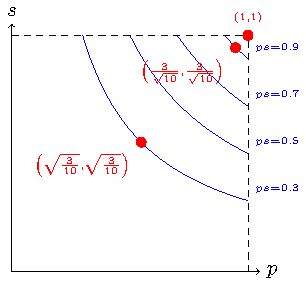
\includegraphics{images/original_space.pdf}}\qquad
	\subfloat[The transformed space for the $k$ nearest neighbours problem.]{\label{fig:knnspace}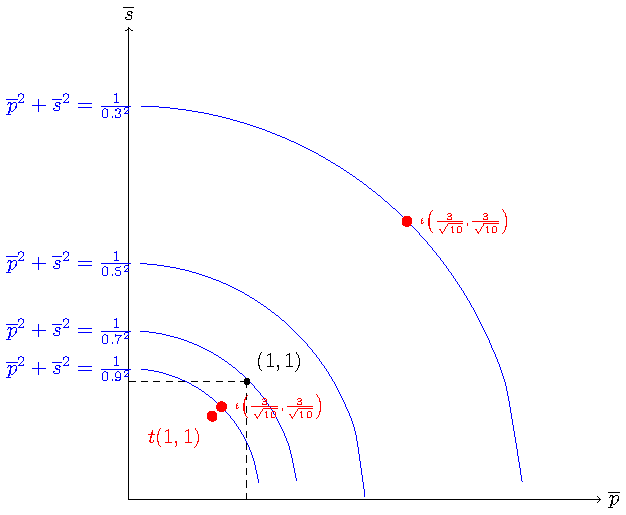
\includegraphics[scale=0.55]{images/transformed_space.pdf}}\\
	\caption{Two different characterizations of the probabilistic trace alignment problem. The best possible match is represented in red in both the similarity/probability space and in the transformed one.}
\end{figure}


 We can show with the next lemma that the following transformation is the one reducing the problem to the $k$-Nearest Neighbour problem:



\begin{lemma}
Given a value $k\in[0,1]\subseteq \mathbb{R}^+_0$, the set of points having the product $ps$ at least $k$ corresponts to the set of $t$-transformed points having a distance of at least $1/k$ from the origin of the axes.
\end{lemma}
\begin{proof}
\[\begin{aligned}
ps\geq k&\Leftrightarrow \frac{1}{ps}\leq\frac{1}{k} \\
	   &\Leftrightarrow \frac{\sqrt{p^2+s^2}}{ps\sqrt{p^2+s^2}}\leq\frac{1}{k} \\
	   &\Leftrightarrow \sqrt{\frac{p^2+s^2}{p^2s^2(p^2+s^2)}}\leq\frac{1}{k} \\
	   &\Leftrightarrow \sqrt{\frac{p^2}{p^2s^2(p^2+s^2)}+\frac{s^2}{p^2s^2(p^2+s^2)}}\leq\frac{1}{k} \\
	   &\Leftrightarrow \sqrt{\frac{1}{s^2(p^2+s^2)}+\frac{1}{p^2(p^2+s^2)}}\leq\frac{1}{k} \\
	   &\Leftrightarrow \left\|{\left({\frac{1}{s\sqrt{p^2+s^2}},\frac{1}{p\sqrt{p^2+s^2)}}\right)}-\vec{0}}\right\|_2\leq\frac{1}{k} \\
	   &\Leftrightarrow \left\|t(p,s)-\vec{0}\right\|_2\leq\frac{1}{k} \\
\end{aligned}\]
\end{proof}
\begin{lemma}
Given a Petri Net $P$ and a trace $t^*$, the probabilistic trace alignment problem of the best $k$ traces reduces to the $k$-Nearest Neighbour problem $\mu_{\tau^*}^{-1}(knn(k,\vec{0},\mu_{\tau^*}(\mathcal{W}_0^{\aleph_0}(P))))$.
\end{lemma}
\begin{proof}
Trivial by definition of $\mu_{\tau^*}$ and for the previous lemma.
\end{proof}

At this stage, we can possibly solve the $k$-probabilistic trace alignment problem by generating a new instance of the $k$-Nearest Neighbour problem for each possible trace $\tau^*$ that we want to align towards the traces coming from a Probabilistic Petri Net. On the other hand, this solution might result quite costly, as solving the problem would require either to use a brute force search algorithm or to load and index our set of points each time.\yellownote{TODO: add references and explaination to the problem (we need a Related Work section\dots? I am accustumed to write such sections.)} In the next section we will discuss an approximated version of the problem providing a trade off between accuracy and efficiency.


\subsection{Approximate $k$-probabilistic Traces Alignment Problem}\label{subsec:akptap}
\texttt{\color{red}[TODO: provide some context and introduction. I'm facing the same problem as in the previous subsection, as the content in here depends on some content that I do not know if I have to write or not\dots]}

Given the characterization of a Probabilistic Petri Net as in \S\ref{subsec:ppn} and the embedding strategy proposed in Definition \ref{def:ppne}, we can generate an embedding for each possible weighted trace $\braket{\tau,w_\tau}\in\mathcal{W}_p^n(P)$ for a given Probabilistic Petri Net $P$ as described in the following definition:
\begin{definition}[Trace Embedding for Probabilistic Petri Nets]
Given a minimum probability threshold $p$, a maximum path length $n$, and a Probabilistic Petri Net $P=(s,t,L,R,w)$ that underwent the $\varepsilon$-closure, we generate the set of the trace embeddings for $P$ as follows:
\begin{enumerate}
	\item for each weighted trace $\braket{\tau,w_\tau}\in\mathcal{W}_p^n(P)$ generated from a path $s\to n_2\rightsquigarrow n_m\to t$ over $R$, we generate a Probabilistic Petri Net $P_\tau=(s',t',L_\tau,R_\tau,w_\tau)$, where \begin{alphalist}
		\item $s'=s$ if $\textit{label}(s)\neq \varepsilon$ and $t'=n_2$ otherwise,
		\item $t'=t$ if $\textit{label}(t)\neq \varepsilon$ and $t'=n_m$ otherwise,
		\item $L_\tau$ (and $R_\tau$) are the projection matrix over the non-$\varepsilon$ labelled notes in $\tau$ and the labels represented in $\tau$,
		\item $w'$ is initialised by $w$ and then multiplied by $[R]_{s,n_2}$ (and $[R]_{m_m,t}$) if $\textit{label}(s)=\varepsilon$ (and  $\textit{label}(t)=\varepsilon$);
	\end{alphalist}
	\item each $P_\tau$ is then represented as $\phi_{\mathcal{P}}(P_\tau)$ and added to the set $\mathbf{T}_p^n(P)$.
\end{enumerate}
\end{definition}

At this stage, the computation of $\underset{\braket{\tau,w_\tau}\in \mathcal{W}_p^n(P), P_\tau\in\mathbf{P}_p^n(P)}{\max\arg} k_{\phi_\mathcal{P}}(P_\tau, T)$ returns the best approximated trace alignment $\tau$ for a query trace represented as $T$. Similarly, we can provide the Probabilistic Petri Net $P\in\mathbf{P}$ providing the best approximated alignment for $T$ as $\underset{P}{\max\arg}\underset{ P_\tau\in\mathbf{P}_p^n(P)}{\max} k_{\phi_\mathcal{P}}(P_\tau, T)$. 
